\part{Hybrid Switched Capacitor LED driver}
\chapter{Hybrid Switched Capacitor Converter}
\label{ch:H-SCC}
Driving high power LEDs using a switched capacitor converter (SCC) challenges the operation of this converter. The SCC provides good performance in voltage-to-voltage conversion, but it can not directly provide regulated current. In low power applications, this is solved by using a linear regulator in series with the LED string, however that is not a valid solution for general lighting where high power and high current are needed. Combining switched capacitors with inductors can provide efficient converters for LED lighting, where the use of an inductor provide a tight and efficient regulation, and the use of switched capacitors allows to reduce the voltage stress in the components, in turn reducing both the switching losses and the volume of the inductor.

The \emph{hybrid} switched capacitor converter (H-SCC), that is introduced in this chapter, is a merge of a switched capacitor and an inductive converter. The first section introduces basic facts about switched capacitor converters (SCC) in order to understand the enhancements, modifications and characteristics of the \emph{hybrid}-SCC. The second section presents the H-SCC topology and  operation. The third section focus in the applications of the H-SCC as a LED driver circuit. Additionally, some driver architectures are described in this section, giving a broader perspective of the possible applications that H-SCC based LED drivers offer.

\section{State of the Art}
In  commercial ICs but also in research the integration and miniaturization characteristics of Switched Capacitor Converters (SCCs) are applied in LED drivers. Commercially there is a large portfolio of available integrated circuits (ICs), designated as Charge-Pumps (CPs), for backlighting in portable devices, \emph{i.e.}  \emph{MAX8930}\footnote{Maxim\textsuperscript{\textregistered} WLED Charge Pump, RGB, OLED Boost, LDOs with ALC and CAI }, \emph{MCP1252/3}\footnote{Microchip\textsuperscript{\textregistered} Low noise, Positive-Regulated Charge Pump}. By merely adding a few external capacitors, these circuits can drive White or RGB LEDs from a Lithium-Ion battery, as shown in the block diagram of Figure~\ref{fig:SCC_backlight_LED}. Generally these chips integrate a SCC with different conversion ratios with a linear regulator for each channel. Various publications ~\cite{07Feng,09Wu,10Yin} propose different modifications of this architecture in order to reduce the parasitic losses, bringing the efficiency close to the theoretical limit. The power ratings of these drivers are below 1$W$ at currents below hundred \emph{milli}-amperes with efficiencies between 70\%-90\% depending on the operation point.

\begin{figure}[!ht]
    \centering
    \begin{circuitikz} [american,scale=0.65]
    \ctikzset{bipoles/length=1cm}
   \draw[thick] (2.5,0.25) --
                (2.5,6.5) --
                (11.5,6.5) --
                (11.5,0.25) --
                (2.5,0.25);

    %Draw SCC block with capacitors
    \draw (3,1) --
          (3,6) --
          (5,6) --
          (5,1) --
          (3,1);

    \draw (4,3) node[rotate=90,anchor=west] {SCC};

    \draw (5,5.5) to[short,-o] (14,5.5);
    \draw (13,5.5) to[capacitor] (13,4.5) node[sground]{};

    \draw (4,1) -- (4,0) node[sground,scale=0.75]{};

   %Draw linear drivers
   \draw  (4,0.5) -- (10.5,0.5) -- (10.5,1);

   %First transitor
   \draw   (10,1) -- (10,1.5) node[npn,anchor=E,scale=0.5](npn1){}
           (npn1.C) -- (10,2.75) to[short,-o] (12,2.75);

   %Second transitor
   \draw  (10,1) -- (11,1)
           node[npn,anchor=E,scale=0.5](npn2){}
           (npn2.C) -- (11,2.25) to[short,-o] (12,2.25);

   %Controller box
   \draw (5.5,1) -- (8.5,1) -- (8.5,3) -- (5.5,3) -- (5.5,1);
   \draw (5.75,2) node[anchor=west, text width = 1.75cm]{Intensity Controller};
   \draw (npn2.B) -| (8.5,2);
   \draw (npn1.B) -| (8.5,2);

   %LEDs

   \draw (14,5.5) to[short,o-] (15,5.5)
                    to[leD*] (15,2.75) to[short,-o] (12,2.75);

   \draw (15,5.5) -- (17,5.5)
                    to[leD*] (17,2.25) to[short,-o] (12,2.25);

   %Add battery

   \draw (-1,0) node[sground,scale=0.75]{} to[battery = $v_{src}$] (-1,5.5)
         -- (3,5.5);

   \draw (3,5) -- (1.5,5) to[C,l_=$c_2$] (1.5,3.5) -- (3,3.5);
   \draw (3,3) -- (1.5,3) to[C,l_=$c_1$] (1.5,1.5) -- (3,1.5);


    \end{circuitikz}
    \caption{Block diagram of the common architecture used in \emph{charge pump} LED drivers for backlighting small screens in portable applications.}
    \label{fig:SCC_backlight_LED}
\end{figure}

With respect to general lighting there are a few research publications that report the use of SCCs. In 2008, ~\citeauthor{08Lee}~\cite{08Lee} presented a step-down converter supplied from rectified 220$V_{rms}$ mains voltage, providing 15W with a 95\% peak efficiency. The proposed architecture directly supplied the LED string from the capacitors, controlling the output power by changing the switching frequency.

In 2012, ~\citeauthor{2012Kline}~\cite{2012Kline} proposed an isolated converter that combined a SCC stage with series-LC resonant converter delivering 15.5W with an efficiency of  92\%.  The SCC stage decreased  the rectified mains voltage, reducing the voltage stress in switches, capacitors, and the resonant tank, allowing to diminish  the volume of the passive components and the total silicon area. The LED current is regulated by modulating both the frequency and the duty cycle.  The architecture was recently implemented in modular silicon dies, allowing to be stacked in order to adjust to different mains voltages~\cite{2013Kline}.


%different LED driver architectures will be presented along with architecture and control modifications that extends the range of operation of the converter.

\section{Switched Capacitor Converter}
%\begin{SCfigure}[][!h]
\begin{wrapfigure}{o}{0.6\textwidth}
    \ctikzset { bipoles/length=1cm}
    \centering
        \begin{circuitikz}[american voltages,scale=0.6]
        \draw
                %Input Supply
                (0,0)  to[V=$v_{src}$]
                %Draw Switches
                (0,7.5)  --
                (5,7.5)  to[switch=$s_1$] %S1
                (5,6)   to[switch=$s_2$] %S2
                (5,4.5)   to[switch=$s_3$] %S3
                (5,3) --
                %left branch
                (3,3)   to[switch=$s_7$]
                (3,1.5)   to[switch=$s_6$]
                (3,0);

        \draw   %right branch
                (5,3) --
                (7,3)   to[switch=$s_4$]
                (7,1.5)   to[switch=$s_5$]
                (7,0) -- (0,0);

        \draw %Capacitor C1
               (3,1.5) -- (2,1.5) -- (2,3)
                to[pC,l_=$c_1$] (2,6) --
               (5,6);

        \draw %Capacitor C2
               (7,1.5) -- (8.25,1.5) --
               (8.25,3) to[pC=$c_2$] (8.25,4.5) --
               (5,4.5);

        \draw %Capacitor C3
               (5,0) to[pC,l_=$c_3$]
               (5,3);

        \draw (7,3) --([hs]8.25,3 |- 7,3) arc(180:0:\radius) to[short,-o] (10,3) to[open,v^=$v_{out}$] (10,0)
        (7,0) to[short,-o] (10,0) node[anchor=west] {};
    \end{circuitikz}
     \caption{3:1 Dickson Converter.}
     \label{fig:demo_full_sch}
\end{wrapfigure}
%\end{SCfigure}
SCCs are a family of SMPS circuits that provide power conversion using only switches and capacitors. %
A SCC has two or more operation modes, referred as phases, and each operating mode is associated with a different circuit arrangement of the capacitors. The SCC is sequentially switching between the different modes, providing a voltage conversion between input and output. The Dickson and Ladder topologies (Figures~\ref{fig:demo_full_sch} and~\ref{fig:31Ladder_sch} respectively) are the preferred SCC topologies used in this dissertation. Both topologies have been selected since they share similar characteristics that favour the design of H-SCCs. Despite the fact that presented examples (in this dissertation) are based on these two topologies, the presented analysis hold for any other well-posed\footnote{The net equations (KVL) of a well-posed converter provides a solvable system with an unique solution for all capacitor voltages. If these voltages cannot be uniquely determined, the converter is not well-posed.} SCC topology~\cite{Seeman:EECS-2009-78}.
%\begin{SCfigure}[][!h]
\begin{wrapfigure}{o}{0.6\textwidth}
    \ctikzset { bipoles/length=1cm}
    \centering
        \begin{circuitikz}[american voltages,scale=0.6]
        \draw
                %Input Supply
                (1,0)  to[V=$v_{src}$]
                %Draw Switches
                (1,9)  --
                (5,9) to[switch=$s_1$] %S1
                (5,7.5) to[switch=$s_1$] %S1
                (5,6)   to[switch=$s_2$] %S2
                (5,4.5) to[switch=$s_3$] %S3
                (5,3)   to[switch=$s_4$]
                (5,1.5) to[switch=$s_5$]
                (5,0) -- (1,0);



        \draw %DC grounded Leg
            (5,0) --
            (7,0) to[pC,l_=$c_5$]
            (7,3) to[pC,l_=$c_3$]
            (7,6) to[pC,l_=$c_1$]
            (7,9) -- (5,9)
            (7,3) -- (5,3)
            (7,6) -- (5,6);

        \draw %Flying Leg
            (5,1.5) --
            (3,1.5) to[pC,l_=$c_4$]
            (3,4.5) to[pC,l_=$c_2$]
            (3,7.5) -- (5,7.5)
            (3,4.5) -- (5,4.5);

        \draw (7,3) to[short,-o]
              (9,3) to[open,v^=$v_{out}$]
              (9,0) to[short,o-] (7,0);

    \end{circuitikz}
     \caption{3:1 Ladder Converter.}
     \label{fig:31Ladder_sch}
\end{wrapfigure}
%\end{SCfigure}
The circuit in Figure~\ref{fig:demo_full_sch} is a two phase 3:1 Dickson converter that provides a step down conversion ratio of $\frac{1}{3}$. During the first phase the odd switches are closed, resulting in the circuit of Figure~\ref{fig:demo_full_p1}. During the second phase, the even switches are closed, resulting in the circuit of Figure~\ref{fig:demo_full_p2}.
\vspace{7cm}
\\
\begin{figure}[!h]
\centering
\ctikzset { bipoles/length=1cm}

    \begin{subfigure}[t]{\textwidth}
    \centering
    %\ctikzset { bipoles/length=1cm}
        \begin{circuitikz}[american voltages,scale=0.6]
        \draw (-1,4) node[anchor=north]{ };
        \draw
                %Input Supply
                (-1,0)  to[V=$v_{src}$]
                %Draw Switches
                (-1,3);
        %Capacitor C1
        \draw   (3,3) -- (2,3) to[pC=$c_1$,v>=$v_1$] (-1,3);

        %Capacitor C2
        \draw (2,0)to[pC=$c_2$,v>=$v_2$](2,3) --(3,3);

        %Capacitor C3
        \draw  (-1,0)--
               (5,0) to[pC=$c_3$,v>=$v_3$]
               (5,3) -- (3,3);

         \draw (5,3) to[short,-o] (6.5,3) node[anchor=west] {};
         \draw (5,0) to[short,-o] (6.5,0) node[anchor=west] {};
         \draw (6.5,3) to[open,v^=$v_{out}$] (6.5,0);
         \end{circuitikz}
     \subcaption{First phase, odd switched are closed and even switches are open.}
     \label{fig:demo_full_p1}
     \end{subfigure}

     \begin{subfigure}[t]{\textwidth}
      \centering
      \begin{circuitikz}[american voltages,scale=0.6]
       \draw (0,5.5) node[anchor=north]{ };
        \draw   %Input Supply
                (-1,0)  to[V=$v_{src}$]
                %Draw Switches
                (-1,4);

        \draw   (5,2) to[pC=$c_2$,v>=$v_2$] (5,4);

        \draw %Capacitor C1
               (2,0)to[pC=$c_1$,v>=$v_1$](2,4) --(5,4);

        \draw %Capacitor C3
               (5,0) to[pC=$c_3$,v>=$v_3$]
               (5,2) ;

         \draw (5,2) to[short,-o] (7.5,2) node[anchor=west] {};
         \draw (-1,0) to[short,-o] (7.5,0) node[anchor=west] {};
         \draw (7.5,1.5) to[open,v^=$v_{out}$] (7.5,0.5);

         %\draw ()
         \end{circuitikz}
     \subcaption{Second phase, even switched are closed and odd switches are open.}
     \label{fig:demo_full_p2}
     \end{subfigure}
\caption{Equivalent circuits of the modes in 3:1 Dickson converter. }
\label{fig:emo_full}
\end{figure}

\subsection{Conversion ratio}
\label{ch:conversion_ratio}
When the converter is unloaded and in steady-state (s.s.), its topology determines the average voltages in the capacitors, and so, its conversion ratio. Therefore, the capacitor s.s. voltages and the conversion ratio of the converter can be obtained by solving a system of linear equations defined by applying Kirchhoff's voltage law (KVL) for each circuit mode. Well-posed converters~\cite{Seeman:EECS-2009-78} provide a solvable system with a unique solution, converters that result in undetermined or overdetermined linear systems are non-well-posed converters and generally require a modification of the converter circuit.

KVL equations of the first phase (see Figure~\ref{fig:demo_full_p1}) are:
\begin{align}
\label{eqn:ph1_kvl}
\begin{split}
  v_{src} - v_{c_1} - v_{c_2} &=0, \\
  v_{out} - v_{c_2}  &=0,\\
  v_{out} - v_{c_3}  &=0.
\end{split}
\end{align}
KVL equations of the second phase (see Figure~\ref{fig:demo_full_p2}) are:
\begin{align}
\label{eqn:ph2_kvl}
\begin{split}
  v_{c_1} - v_{c_2} - v_{c_3} &=0, \\
  v_{out} - v_{c_3}  &=0.
\end{split}
\end{align}
Selecting the linear independent equations from (\ref{eqn:ph1_kvl}) and (\ref{eqn:ph2_kvl}), a solvable system can be formulated as
\begin{equation}
  \syssubstitute{.,{a_1}{v_{src}}{a_2}{v_{out}}{b_1}{v_{c1}}{b_2}{v_{c2}}{b_3}{v_{c3}}}
  \systeme{
    a_1  - b_1 -b_2  = 0,
    b_1 - b_2 - b_3  = 0,
    b_2   = a_2,
    b_3  =  a_2}.
    \label{eqn:sys_kvl}
\end{equation}
%\begin{align}
%\begin{split}
%  v_{src} - v_{c_1} - v_{c_2} &=0, \\
%  v_{c_1} - v_{c_2} - v_{c_3} &=0, \\
%  v_{out} - v_{c_2}  &=0,\\
%  v_{out} - v_{c_3}  &=0,
%\end{split}
%\end{align}
Solving it results in
\begin{align}
\label{eqn:sol_kvl}
\begin{split}
  v_{out} =  v_{c_3} = v_{c_2} &=\frac{V_{src}}{3} , \\
  v_{c_1} &=\frac{2 \cdot V_{src}}{3} ,
\end{split}
\end{align}
hence the converter conversion ratio is
\begin{equation}
\label{eqn:m_kvl}
m_i = \frac{v_{out}}{v_{src}} = \frac{1}{3}.
\end{equation}

The results show that unloaded conversion ratio is defined by the topology of the converter and independent of the switching operating regime (frequency and duty cycle). From here on, the topology defined conversion ratio will be referred to as the \emph{intrinsic} conversion ratio $m_i$.

\subsection{Output voltage regulation}
As previously demonstrated, a SCC has a fixed conversion ratio only defined by its topology and not by its operation regime, therefore the converter can not directly provide voltage regulation.
\begin{SCfigure}[][!h]
%\begin{wrapfigure}{o}{0.6\textwidth}
\centering
\ctikzset { bipoles/length=1cm}
\tikzstyle{block} = [draw, rectangle, fill=white!40]
\begin{circuitikz} [american voltages, scale=0.65]
\draw   (-3,0) --
        (-4,0) to[V = $v_{src}$]
        (-4,3) -- (-3,3);

 \draw  (0.5,3) to[open,v^=$m_i \cdot v_{src} $] (0.5,0);

 \draw  (0,3)  to[generic,v^=$v_{drop}$,i_=$i_o$]
        (4,3)  to[R,l_=$r_l$,v^=$v_{out}$]
        (4,0) -- (0,0);

 \node [block] (SCC) [minimum height = 2.6cm, minimum width = 1.95cm] at(-1.5,1.5) {SCC};
 %\node [block] (SCC) [minimum height = 4pt, minimum width = 3pt] at(-.5,1.5) {SCC};
\end{circuitikz}
\caption[Linear regulated SCC]{Conceptual block diagram of a linear regulated switched capacitor.}
\label{fig:linear_scc}
%\end{wrapfigure}
\end{SCfigure}
Indirectly, there is always the possibility to regulate the output voltage by means of a linear regulator, thus the output voltage is adjusted by drooping the excess voltage ($v_{drop}$) in a series element with the load, as shown in the schematic of Figure~\ref{fig:linear_scc}. This can be achieved in two ways: Using an external linear regulator connected  between the converter output and the load, or what is more common, using or \emph{'misusing'}  the behaviour of the SCC in order to provide this linear regulation characteristic~\cite{Ng:EECS-2011-94} . Both ways of regulation reduces the efficiency of the converter. Like in a linear regulator~\eqref{eq:linear_reg},  the efficiency of the converter can be written as a function of $v_{src}$ and $v_o$, giving
\begin{equation}
\eta = \frac{P_o}{P_i} = \frac{v_o \cdot i_o}{m_i \cdot v_{src} \cdot i_o} = \frac{v_o}{m_i \cdot v_{src}}.
\label{eq:eff_vo}
\end{equation}
\begin{SCfigure}[][!h]
\centering
\begin{circuitikz}
    \begin{scope}%[xshift = 8cm, yshift=0cm]
        \draw[->] (0,0) -- (4,0) node[anchor=south] {$  m_e $};
        \draw[->] (0,0) -- (0,4) node[anchor=east] {$\eta $};

        %Ticks X
        \draw (3,2pt) -- (3,-5pt)  node[anchor=north west] {$1$};
        \draw (1.5,2pt) -- (1.5,-5pt)   node[anchor=north west] {$\frac{1}{2}$};

        %Ticks Y
        \draw (2pt,3) -- (-5pt,3) node[anchor=east] {$100\%$};
        \draw (2pt,1.5) -- (-5pt,1.5) node[anchor=east] {$50\%$};

        %Markers
        \draw[dotted] (3,3) -- (3,0);
        \draw[dotted] (3,3) -- (0,3);
        \draw[dotted] (1.5,3) -- (1.5,0);
        \draw[dotted] (1.5,1.5) -- (0,1.5);


        \draw[thick,dashed] (3,3) -- (0,0);
        \draw[thick] (1.5,3) -- (0,0);

        \draw[thick] (0.75,4) -- (1.25,4) node[anchor=west] {Linear regulator};
        \draw[thick,dashed] (0.75,3.5) -- (1.25,3.5) node[anchor=west] {2:1 SCC};
\end{scope}
\end{circuitikz}
\caption[Efficiency comparison between a linear regulator and a SCC]{Maximum theoretical efficiency plotted as function of the \emph{effective} conversion ratio: \emph{dashed line} - linear regulator; \emph{thick line} - linear regulated 2:1 SCC.}
\label{fig:eff_crv_linear_vs_scc_linear}
\end{SCfigure}
In order to compare the efficiencies among different converters, we define the \emph{effective conversion ration} ($m_e$ ) as the ratio between the voltage source and the load, thus
\begin{equation}
m_e = \frac{v_{out}}{v_{src}} \label{eq:eff_m}
\end{equation}
Figure~\ref{fig:eff_crv_linear_vs_scc_linear} compares the efficiency of a linear regulator and a linear regulated 2:1 SCC, showing that below $m_e=1/2$ the 2:1 SCC has better efficiency, however above $1/2$ the SCC is not longer operative. Anyway in both cases the efficiency drops as the output voltages decreases. 
%\vspace{5cm}

\subsection{Multiple conversion ratio converters}
%\begin{wrapfigure}{o}{0.6\textwidth}
Multiple conversion ratio converters enable to extend the regulation margins and increase the conversion efficiency. Figure~\ref{fig:eff_crv_linear_vs_scc_linear} shows the limitations of a 2:1 SCC. First, the converter is only operative for \emph{effective} conversion rations ($m_e$) below $1/2$. Second, as $m_e$ moves below the intrinsic conversion ratio of the converter ($m_i=1/2$) the efficiency decreases linearly.
Other topologies, like the one of Figure~\ref{fig:M_SCC_ckt}, have multiple \emph{intrinsic} conversion ratios - $\frac{1}{3}$, $\frac{1}{2}$, $\frac{2}{3}$ and $1$ - that extend the operation margins and increase the efficiency of the converter as shown in the plot of Figure~\ref{fig:M_SCC_plt}.
\begin{figure}[!h]
    \centering
    \parbox[b]{.45\linewidth}{
            \raggedright
            \ctikzset { bipoles/length=1cm}
\begin{circuitikz} [american,scale=0.65]
    %\draw (0,7) node[anchor=south] {};
    \draw
        (0.5,-4) node[sground] {} to[V = $v_{src}$] (0.5,-2)
        (0.5,3) to[gswitch=$s_1$]
        (2.5,3) to[capacitor=${c_1}$]
        (3.5,3) -- (5,3) to[gswitch=$s_2$]
        (6.5,3);

    %Switch s9
    \draw (4,3) -- (4,1.5) to[gswitch=$s_9$] (2,1.5) -- (2,-2);

    %Switch s4
    \draw (5,3)  to[gswitch=$s_4$] (5,1.5) node[sground] {} ;

    %Switch branch to load
    \draw (2.25,3) --
          (2.25,4.5) to[gswitch=$s_3$]
          (6.5,4.5) -- (6.5,-2);

    \draw (0.5,3) -- (0.5,-2) to[gswitch=$s_5$] (2,-2) -- (2.5,-2) to[capacitor=${c_2}$] (3.5,-2) -- (4,-2) to[gswitch=$s_6$] (6.5,-2);

    %Switch s7
    \draw (2,-0.5) to[gswitch,l^=$s_7$] (6.5,-0.5);

    %Switch s8
    \draw (4,-2)  to[gswitch,l_=$s_8$] (4,-4) node[sground] {} ;


    %Load and capacitor C2
    \draw (6.5,-4) node[sground]{} to[capacitor,l^=$c_o$] (6.5,-2);

    \draw (6.5,-2) to[short,-o] (7.5,-2) node[anchor=west] {$v_o$};
\end{circuitikz}

            \subcaption{Circuit schematic}
            \label{fig:M_SCC_ckt}
    }
    \hfill
    \parbox[b]{.45\linewidth}{
            \raggedleft
            \ctikzset { bipoles/length=1cm}
\begin{circuitikz}
    \begin{scope}[xscale=0.75, yscale=0.85]
        \draw (0,4.5) node[anchor=south] {};
        \draw[->] (0,0) -- (7,0) node[anchor=south] {$  m_e $};
        \draw[->] (0,0) -- (0,4) node[anchor=east] {$\eta $};

        %Ticks X
        \draw (6,2pt) -- (6,-5pt)  node[anchor=north  ] {$1$};
        \draw (3,2pt) -- (3,-5pt)   node[anchor=north ] {$\frac{1}{2}$};
        \draw (4,2pt) -- (4,-5pt)   node[anchor=north ] {$\frac{2}{3}$};
        \draw (2,2pt) -- (2,-5pt)   node[anchor=north ] {$\frac{1}{3}$};
        \draw (0,0) node[anchor=north east] {$0$};

        %Ticks Y
        \draw (2pt,3) -- (-5pt,3) node[anchor=east] {$100\%$};
        \draw (2pt,1.5) -- (-5pt,1.5) node[anchor=east] {$50\%$};

        %Markers
        \draw[dotted] (6,3) -- (6,0);
        \draw[dotted] (6,3) -- (0,3);
        \draw[dotted] (3,3) -- (3,0);
        \draw[dotted] (3,1.5) -- (0,1.5);


        \draw[thick,dashed] (6,3) -- (0,0);
        \draw[thick] (0,0)--(2,3)--(2,2) -- (3,3) -- (3,2.25) -- (4,3) -- (4,2) -- (6,3);

        \draw[thick] (0.75,4) -- (1.25,4) node[anchor=west,font=\footnotesize]  { Multi-target SCC};
        \draw[thick,dashed] (0.75,3.5) -- (1.25,3.5) node[anchor=west,font=\footnotesize] {Linear regulator};

    \end{scope}
\end{circuitikz} 
            \subcaption{Maximum theoretical efficiency.}
            \label{fig:M_SCC_plt}
    }
    \caption{Multiple conversion ratio converter.}
    \label{fig:M_SCC}
\end{figure}

\subsection{Converter output nodes}
The previous section presented switched capacitor converters with the load connected to a node that provides a fixed conversion ratio. Actually, that is the most common way of employing these converters, however a SCC can supply the load from other nodes. As shown in Figure~\ref{fig:dc_pwm_nodes}, two different types of nodes can be identified: \emph{node a} -  fixed voltage \emph{dc}-node; \emph{node b} - floating voltage \emph{pulse width modulated} node (\emph{pwm}-nodes).
\begin{figure}[!h]
\centering
\ctikzset { bipoles/length=1cm}
\begin{circuitikz}[american voltages,scale=0.65]
\draw
        %Draw Switches
        (1.5,0)  to[V=$v_{src}$]
        (1.5,6)  --
        (5,6)   to[switch=$s_1$]
        (5,4.5)   to[switch=$s_2$]
        (5,3)   to[switch=$s_3$]
        (5,1.5)   to[switch=$s_4$]
        (5,0)  --
        (1.5,0)

        (5,4.5) to[short,-o]
        (8,4.5) node[anchor=west] {$b \rightarrow$  \emph{pwm}  node}

        (5,3) to[short,-o]
        (8,3) node[anchor=west] {$a \rightarrow$ \emph{dc} node}

%Draw Capacitors
        (5,1.5) --
        (3,1.5) to[C,l_=$c_{fly}$]
        (3,4.5)--
        (5,4.5)

        (5,0) --
        (7,0) to[C=$c_{dc}$,mirror]
        (7,3)--
        (5,3);

  \begin{scope}[xshift=13cm,yshift=0.2cm]
  \draw [->] (-0.1,0) -- (5,0) node[anchor=west]{$t$};
  \draw [->] (0,-0.1) -- (0,2.5) node[anchor=east]{$v_a$};
  %\draw (0,-1) node[anchor=south]{0}
%        (1.25,-1) node[anchor=south] {$T$}
%        (2.5,-1)  node[anchor=south] {$2T$}
%        (3.75,-1) node[anchor=south] {$3T$} ;

  \draw [thick] (0,1) -- (0.75,0.75) -- (0.75,0.95) -- (1.25,0.80)
                      -- (1.25,1)-- (2,0.75) -- (2,0.95) -- (2.5,0.80)
                      -- (2.5,1)-- (3.25,0.75) -- (3.25,0.95) -- (3.75,0.80);

  \draw [dashed] (0,0.875) -- (4,0.875) node[anchor=west]{$v_a$} ;
  \end{scope}

  \begin{scope}[xshift=13cm,yshift=4 cm]
  \draw [->] (-0.1,0) -- (5,0) node[anchor=west]{$t$};
  \draw [->] (0,-0.1) -- (0,2.5) node[anchor=east]{$v_b$};
  %\draw (0,-1) node[anchor=south]{0}
%        (1.25,-1) node[anchor=south] {$T$}
%        (2.5,-1)  node[anchor=south] {$2T$}
%        (3.75,-1) node[anchor=south] {$3T$} ;

  \draw [thick] (0,2) -- (0.75,1.85) -- (0.75,1) -- (1.25,0.80) --
                (1.25,2) -- (2,1.85) -- (2,1) -- (2.5,0.80) --
                (2.5,2)-- (3.25,1.85) -- (3.25,1) -- (3.75,0.80);

  \draw [dashed] (0,1.515) -- (4,1.515) node[anchor=west]{$v_b$} ;
  \end{scope}

\end{circuitikz}
\caption[Nodes types in a SCC]{Node types in a 2:1 converter: Node $a$ is a \emph{dc}-node; its voltage, $v_a$ is plotted in the bottom graph. Node $b$ is a \emph{pwm}-node; its voltage, $v_b$, is plotted in the top graph.}
\label{fig:dc_pwm_nodes}
\end{figure}

Fixed voltage \emph{dc}-nodes are the common output nodes of a SCC. A \emph{dc}-node supplies the load with a fixed conversion ratio defined by the topology, and  with a low voltage ripple thanks to the capacitor in parallel with the load. The capacitors that are connected between a \emph{dc}-node and ground are  \emph{dc}-capacitors as shown in Figure \ref{fig:dc_pwm_nodes}. A SCC can have one or more \emph{dc}-capacitors. Topologies that reduce the number of \emph{dc}-capacitors trend to have a better capacitor utilization, since these capacitors do not contribute to transport charge~\cite{Seeman:EECS-2009-78}.

The use of floating \emph{pulse width modulated}-nodes (\emph{pwm}-nodes) was not reported until a couple of recent publications~\cite{2012Kumar, 2012Kline} presented the advantages of using them. \emph{Pwm}-nodes were considered internal to the converter without any added functionality, nevertheless the conversion possibilities of SCCs can be further enhanced by using these nodes as outputs for the converter. \emph{Pwm}-nodes are accessible from the terminals of flying capacitors ($c_{fly}$), delivering a floating pulse-width-modulated (PWM) voltage with an added \emph{dc} offset of a fraction of the input voltage with respect to ground. The magnitudes are related to the SCC topology. The pulsating voltages can be filtered using an inductive-capacitive filter (\emph{LC}), allowing to supply a \emph{dc} load with the averaged voltage of the node. Furthermore the \emph{pwm} voltage at the node can be controlled by adjusting the duty
cycle of the SCC, enhancing the regulation capabilities of these outputs compared to the fixed conversion ration of the \emph{dc}-nodes.

\section{Hybrid-Switched Capacitor Converter}
\begin{SCfigure}[][!h]
\ctikzset { bipoles/length=1cm}
\centering
    \begin{circuitikz}[american,scale=0.6]

    \draw
            %Input Supply
            (0,0)  to[V=$v_{src}$]
            %Draw Switches
            (0,7.5)  --
            (5,7.5)  to[switch=$s_1$] %S1
            (5,6)   to[switch=$s_2$] %S2
            (5,4.5)   to[switch=$s_3$] %S3
            (5,3) --
            %left branch
            (3,3)   to[switch=$s_7$]
            (3,1.5)   to[switch=$s_6$]
            (3,0);

    \draw   %right branch
            (5,3) --
            (7,3)   to[switch,l_=$s_4$]
            (7,1.5)   to[switch,l_=$s_5$]
            (7,0) -- (0,0);

    % Nodes
    \draw   (5,6) node[anchor=west] {$n_1$};
    \draw   (5,4.5) node[anchor=east] {$n_2$};
    \draw   (2,1.5) node[anchor=east] {$n_3$};
    \draw   (8.25,1.5) node[anchor=west] {$n_4$};



    \draw %Capacitor C1
           (3,1.5) -- (2,1.5)
            to[pC,l_=$c_1$] (2,6) --
           (5,6);

    \draw %Capacitor C2
           (7,1.5) --
           (8.25,1.5)  to[pC,l_=$c_2$](8.25,4.5) --
           (5,4.5);

    \draw  %Inductor
            (8.25,4.5) to[L=$l_o$,-o] (12,4.5);


    \draw %Capacitor C3
           (5,0) to[pC,l_=$c_3$] (5,3);

     %\draw (7,4) to[short,-o] (10,4) node[anchor=west] {};
     \draw (7,0) to[short,-o] (12,0) node[anchor=west] {};
     \draw (12,4.5) to[open,v^=$v_{out}$] (12,0);
     \draw (8.25,4.5) node[anchor=south] {$v_x$};

     \draw (11.5,0) to[pC,l=$c_{o}$] (11.5,4.5);

     \end{circuitikz}
 \caption{ A 3:1 H$^2$-Dickson topology with the inductor connected to the second \emph{pwm}-node.}
 \label{fig:3_1_hscc}
\end{SCfigure}
A Hybrid Switched Capacitor Converter (H-SCC) uses a low pass filter to supply a \emph{dc} voltage from a \emph{pwm}-node.  Figure~\ref{fig:3_1_hscc} shows the \emph{hybrid} configuration of the 3:1 Dickson converter, where the output filter is connected to the node $n_2$. The low pass filter is composed of an inductor $l_o$ and capacitor $c_o$, and removes high frequency \emph{ac}-component present in the node. From this point on the \emph{hybrid} variation of a SCC topology will be denoted by adding an H$^x$ in front of the topology's name, where the superscript refers to the used output, thus  the converter in Figure~\ref{fig:3_1_hscc} is now referred as 3:1 H$^2$-Dickson.
\begin{SCfigure}[][!h]
\centering
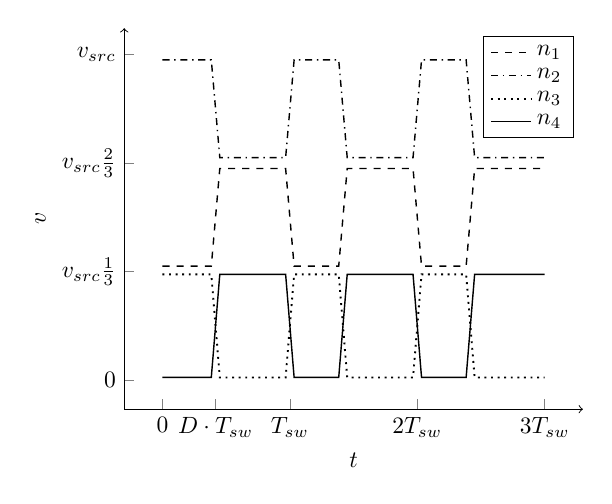
\begin{tikzpicture}[xscale=0.85, yscale=0.85]
    \begin{axis}[
        xlabel near ticks,
        xlabel=$t$,
        ylabel=$v$,
        axis line style={->},
        axis y line*=left,
        axis x line*=bottom,
        ytick = {0,2,4,6},
        yticklabels={0,$v_{src}\frac{1}{3}$,$v_{src}\frac{2}{3}$,$v_{src}$},
        xtick = {0,1.25,3,6,9},
        xticklabels={0,$D \cdot T_{sw}$,$T_{sw}$ ,$2 T_{sw}$,$3 T_{sw} $},
        ]

  %Vertical ticks
  %\draw (2pt,6) -- (-5pt,6) node[anchor=east]  {$v_{src} $};
  %\draw (2pt,4) -- (-5pt,4) node[anchor=east]  {$v_{src} \frac{2}{3}$};
  %\draw (2pt,2) -- (-5pt,2) node[anchor=east]  {$v_{src} \frac{1}{3}$};

  %Horizontal ticks
  %\draw (1.25,2pt) -- (1.25,-5pt) node[anchor=north]  {$DT$};
  %\draw (3,2pt) -- (3,-5pt) node[anchor=north]  {$T$};
  %\draw (6,2pt) -- (6,-5pt) node[anchor=north]  {$2T$};
  %\draw (9,2pt) -- (9,-5pt) node[anchor=north]  {$3T$};
  %\draw (0,0) node[anchor=north east]  {$0$};

  \addplot[semithick, dashed]
    plot coordinates{
        (0,2.1)   (1.15,2.1)  (1.35,3.9)  (2.9,3.9)
        (3.1,2.1) (4.15,2.1)  (4.35,3.9)  (5.9,3.9)
        (6.1,2.1) (7.15,2.1)  (7.35,3.9)  (9,3.9) };

  \addplot[semithick, dashdotted ]
    plot coordinates{
     (0,5.9)    (1.15,5.9)  (1.35,4.1)  (2.9,4.1)
     (3.1,5.9)  (4.15,5.9)  (4.35,4.1)  (5.9,4.1)
     (6.1,5.9)  (7.15,5.9)  (7.35,4.1)  (9,4.1)} ;

  \addplot[thick,dotted ]
    plot coordinates{
   (0,1.95)   (1.15,1.95)  (1.35,0.05)  (2.9,0.05)
   (3.1,1.95) (4.15,1.95)  (4.35,0.05)  (5.9,0.05)
   (6.1,1.95) (7.15,1.95)  (7.35,0.05)  (9,0.05)};

   \addplot[semithick]
    plot coordinates{
    (0,0.05)    (1.15,0.05)    (1.35,1.95)    (2.9,1.95)
    (3.1,0.05)  (4.15,0.05)  (4.35,1.95)  (5.9,1.95)
    (6.1,0.05)  (7.15,0.05)  (7.35,1.95)  (9,1.95) };

    \legend{$n_1$,$n_2$,$n_3$,$n_4$}


\end{axis}
\end{tikzpicture}
\caption{Transient voltage at the different \emph{pwm}-nodes of the 3:1 H-Dickson converter of Figure~\ref{fig:3_1_hscc}.}
\label{fig:pwm_nodes}
\end{SCfigure}
For sake of clarity, the operation of a H-SCC is illustrated using the 3:1 Dickson converter used previously, which the steady-state (s.s.) voltages where already solved in Section~\ref{ch:conversion_ratio}. Except for the added filter, the SCC topology keeps the same circuit structure as in the original converter, and so they do the s.s. voltages in the capacitors. The two switching modes of the converter are shown in Figures~\ref{fig:3_1_hscc_p1} and~\ref{fig:3_1_hscc_p2}, displaying the voltages values of the capacitors. Through a graphical inspection, it can be seen that the voltage at the switching node $v_x$ is different in each switching cycle, producing the \emph{pwm}-voltage shown in Figure~\ref{fig:vx_t}. The unloaded voltage at the switching node $v_x$ over an entire switching period $T_{sw}$ is defined with a discontinuous function as
\begin{equation}
v_x(t) = \left\{
\begin{array}{lcccccr}
  \frac{1}{3} v_{src}   & : & 0   & < & t & \leq & D  T_{sw}  \\
  ~\\
   \frac{2}{3} v_{src} & : & D T_{sw} & < & t & \leq & T_{sw},
\end{array}
\right.
\label{eq:vx_t}
\end{equation}
where $D$ corresponds to the duty cycle of the odd switches.
\begin{figure}[!h]
    \begin{subfigure}{0.4\textwidth}
    \ctikzset { bipoles/length=1cm}
    \centering
    \begin{circuitikz}[american,scale=0.6]
    \draw
            %Input Supply

            %Draw Switches
            (5,8) node[anchor=south] {$v_{src}$}
            (5,7.5) node[rground, yscale=-1] {}
            (5,7.5)  to[cswitch=$s_1$] %S1
            (5,6)   to[switch=$s_2$] %S2
            (5,4.5)   to[cswitch=$s_3$] %S3
            (5,3) --
            %left branch
            (3,3)   to[cswitch,l_=$s_7$]
            (3,1.5)   to[switch,l_=$s_6$]
            (3,0);

    \draw   %right branch
            (5,3) --
            (7,3)   to[switch,l=$s_4$]
            (7,1.5)   to[cswitch,l=$s_5$]
            (7,0) -- (3,0);


    \draw %Capacitor C1
           (3,1.5) -- (2,1.5)
            to[pC,l_=$c_1$,v^>=$\frac{2 v_{src}}{3}$] (2,6) --
           (5,6);

    \draw %Capacitor C2
           (7,1.5) --
           (8.25,1.5) -- (8.25,2) to[pC,l=$c_2$,v>=$\frac{v_{src}}{3}$](8.25,4.5) --
           (5,4.5);



    \draw %Capacitor C3
           (5,0) node[sground] {} to[pC,l_=$c_3$,v^>=$\frac{v_{src}}{3}$] (5,3);

     %\draw (7,4) to[short,-o] (10,4) node[anchor=west] {};
     \draw (8.25,4.5) to[short,-o] (9.25,4.5) node[anchor=south,] {$v_x$};


     \end{circuitikz}
     \subcaption{Phase 1: Odd switches closed.}
     \label{fig:3_1_hscc_p1}
  \end{subfigure}
  \hfill
    \begin{subfigure}{0.4\textwidth}
    \ctikzset { bipoles/length=1cm}
    \centering
    \begin{circuitikz}[american,scale=0.6]
    \draw
            %Input Supply

            %Draw Switches
            (5,8) node[anchor=south] {$v_{src}$}
            (5,7.5) node[rground, yscale=-1] {}
            (5,7.5)  to[switch=$s_1$] %S1
            (5,6)   to[cswitch=$s_2$] %S2
            (5,4.5)   to[switch=$s_3$] %S3
            (5,3) --
            %left branch
            (3,3)   to[switch,l_=$s_7$]
            (3,1.5)   to[cswitch,l_=$s_6$]
            (3,0);

    \draw   %right branch
            (5,3) --
            (7,3)   to[cswitch,l=$s_4$]
            (7,1.5)   to[switch,l=$s_5$]
            (7,0) -- (3,0);


    \draw %Capacitor C1
           (3,1.5) -- (2,1.5)
            to[pC,l_=$c_1$,v^>=$\frac{2 v_{src}}{3}$] (2,6) --
           (5,6);

    \draw %Capacitor C2
           (7,1.5) --
           (8.25,1.5) -- (8.25,2) to[pC,l=$c_2$,v>=$\frac{v_{src}}{3}$](8.25,4.5) --
           (5,4.5);



    \draw %Capacitor C3
           (5,0) node[sground] {} to[pC,l_=$c_3$,v^>=$\frac{v_{src}}{3}$] (5,3);

     %\draw (7,4) to[short,-o] (10,4) node[anchor=west] {};
     \draw (8.25,4.5) to[short,-o] (9.25,4.5) node[anchor=south,] {$v_x$};


     \end{circuitikz}
     \subcaption{Phase 2: Even switches closed.}
     \label{fig:3_1_hscc_p2}
  \end{subfigure}

 \caption[Two switching phases of 3:1 H-Dickson$^2$]{ Two switching phases of \emph{hybrid} 3:1 Dickson loaded at the second node.}
 \label{fig:3_1_hscc_phases}
\end{figure}
The output filter averages the voltage at the switching node $v_x$, therefore the mean value at $v_{out}$ can be obtained by integrating~\eqref{eq:vx_t} over an entire switching cycle,
\begin{align}
 v_{out} & = \frac{1}{T} \int_{0}^{T}  v_x(t) dt \\[3ex]
 v_{out} & = \frac{1}{T} \left( \int_{0}^{DT} \frac{1}{3} v_{src} ~dt + \int_{DT}^{T} \frac{2}{3} v_{src} ~dt \right) \\[3ex]
 v_{out} & = \frac{2-D}{3} v_{src},
 \label{eq:int_vx_t}
\end{align}
thus the intrinsic conversion ratio of the converter for the second node ($n_2$) is
\begin{equation}
 m_2   = \frac{v_{out}}{v_{src}} = \frac{2-D}{3},
 \label{eq:int_vx_t}
\end{equation}
where the subscript in $m$ denotes the node of the converter. The numbering of the nodes is done from  top-bottom to left-right, see the circuit schematic of Figure~\ref{fig:3_1_hscc}.
\begin{SCfigure}[][!h]
\centering
\begin{circuitikz}[american voltages,xscale=0.55,yscale=0.65]
\begin{scope}
  \draw [->] (0,0) -- (10,0) node[anchor=west]{$t$};
  \draw [->] (0,0) -- (0,5.5) node[anchor=east]{$v_x$};

  %Vertical ticks
  \draw (2pt,4) -- (-5pt,4) node[anchor=east]  {$v_{src} \frac{2}{3}$};
  \draw (2pt,2.5) -- (-5pt,2.5) node[anchor=east]  {$v_{src} \frac{1}{3}$};

  %Horizontal ticks
  \draw (1.25,2pt) -- (1.25,-5pt) node[anchor=north]  {$DT$};
  \draw (3,2pt) -- (3,-5pt) node[anchor=north]  {$T$};
  \draw (6,2pt) -- (6,-5pt) node[anchor=north]  {$2T$};
  \draw (9,2pt) -- (9,-5pt) node[anchor=north]  {$3T$};
  \draw (0,0) node[anchor=north east]  {$0$};

  \draw[thick] (0,2.5) -- (1.25,2.5) -- (1.25,4) -- (3,4) --
               (3,2.5) -- (4.25,2.5) -- (4.25,4) -- (6,4) --
               (6,2.5) -- (7.25,2.5) -- (7.25,4) -- (9,4) ;

  \draw[thick, dashed] (0,3.375) -- (7.25,3.375) ;
  \draw (2.075,3.375)node[anchor=north] {$\bar{v_x}$};

  \draw[pil,<->] (8,4.1) -- (8,2.4) ;

  \draw[dotted] (7.25,2.5) -- (8.1,2.5);

  \draw (8,3.25) node[anchor=west] {$\Delta v_x$};
\end{scope}
\end{circuitikz}
\caption{Transient voltage at the switching node of the switching node $v_x$ of the H-SCC in Figure~\ref{fig:3_1_hscc}}
\label{fig:vx_t}
\end{SCfigure}

In the 3:1 H$^2$-Dickson there is actually a plurality of \emph{pwm}-nodes. Figure~\ref{fig:pwm_nodes} plots all the switching voltages available in the converter. The square-wave voltages cover the range from 0 to $v_{src}$ in equal steps of $v_{src}/3$. This equal spacing is one of the features of Dickson and Ladder converters, and the reason why these two topologies were selected to implement all the H-SCCs discussed in this dissertation. An advantage of this equal spacing is that for the same inductor value, the inductor current ripple stays the same independently to used \emph{pwm}-node. In fact, the amplitude of the PWM voltage in any Dickson and Ladder converters at the switching node is fixed by the intrinsic conversion ratio $m_i$, thus
\begin{equation}
\Delta v_{x} = m_i v_{src}.
\label{eq:del_vx}
\end{equation}

A H-SCC shares many of the characteristics of a buck converter, which is the most common \emph{dc-dc} topology used as a LED driver. Adding the output filter to a SCC complements the converter by providing tight current regulation, which overcomes the intrinsic limitation of SCC in this respect. However, it requires magnetic elements, challenging the integrability  of the converter. The following sections introduce the characteristics of this new \emph{hybrid} topology as a LED driver, using the buck converter as a reference. %  since a H-SCC architecture can directly replace a buck converter LED driver providing the same regulation characteristics.

\subsection{Output Regulation}
\label{sec:out_reg}
In contrast with the classical SCC, the conversion ratio of a H-SCC converter can be adjusted. It actually depends on the duty cycle ($D$) of the driving signals, and consequently the conversion ratio can be adjusted to provide regulation to the load without directly affecting the converter's efficiency.

Figure~\ref{fig:reg_comp} compares the trend curves of the converter efficiency with respect to the conversion ratio for a three different converters a 3:1 H$^3$-Dickson, a 3:1 Dickson and a buck converter. For instance, the \emph{dc}-node of the 3:1 Dickson has an intrinsic conversion ratio of $m_i = \frac{1}{3} $, and it provides regulation at the cost of efficiency. Instead using the third \emph{pwm}-node ($n_3$) of the same Dikson converter of Figure~\ref{fig:3_1_hscc}, the converter has an adjustable conversion ratio given by
\begin{equation}
m_3 = \frac{D}{3}
\end{equation}
where $D$ is the duty cycle of the odd numbered switches. In this case the efficiency-regulation ($\eta$-$m_e$) curve is flat within the regulation margins, and drops for extreme duty cycles because of, not yet discussed\footnote{The details of the loss mechanisms in SCC and H-SCC are covered in Chapter~\ref{ch:modeling} dedicated to modeling.}, internal losses of the SCC stage. Furthermore, the $\eta$-$m_e$ curve of a H-SCC is similar to the one of a buck converter but with a smaller dynamic range.
\begin{SCfigure}[][!h]
\centering
\begin{circuitikz}[american,xscale=0.55,yscale=0.65]
\begin{scope}


  \draw [->] (0,0) -- (10,0) node[anchor=north]{$m_e$};
  \draw [->] (0,0) -- (0,5.5) node[anchor=east]{$\eta$};

  %Vertical ticks
  \draw (2pt,4) -- (-5pt,4) node[anchor=east]  {$100\%$};
  \draw (2pt,2.5) -- (-5pt,2.5) node[anchor=east]  {$70\%$};

  %Horizontal ticks
  %\draw (1.25,2pt) -- (1.25,-5pt) node[anchor=north]  {$DT$};
  \draw (3,2pt) -- (3,-5pt) node[anchor=north]  {$\frac{1}{3}$};
  \draw (6,2pt) -- (6,-5pt) node[anchor=north]  {$\frac{2}{3}$};
  \draw (9,2pt) -- (9,-5pt) node[anchor=north]  {$1$};
  \draw (0,0) node[anchor=north east]  {$0$};

  \draw[thick, dashed] (0,0) --  (2.9,3.9) ;

  %\draw[thick, dotted] (0,0) --  (2.9,3.9) ;
  \draw[thick,dotted] (0.1,2) parabola[bend at end] (2,3.45) -- (6,3.7) parabola[bend at start] (8.9,1.5);

  \draw[thick] (0.1,1.75) parabola[bend at end] (0.75,3.5) -- (2.2,3.6) parabola[bend at start] (2.9,1.6);

  \draw[thick] (4,5) -- (5,5) node[anchor=west,font=\small] {3:1 H$^3$-Dikson};
  \draw[thick,dashed] (4,4.5) -- (5,4.5) node[anchor=west,font=\small] { 3:1 Dickson };
  \draw[thick,dotted] (4,5.5) -- (5,5.5) node[anchor=west,font=\small] { Buck };
\end{scope}
\end{circuitikz}
\caption{Comparison of regulation-efficiency characteristics between converters.}
\label{fig:reg_comp}
\end{SCfigure}

\begin{table}[h]

\centering
\caption{Intrinsic conversion ratios, $m_i$, at the different nodes of a 3:1 H-Dickson converter.}
\label{tab:3:1 H-Dick_M}
\renewcommand{\arraystretch}{1.5}% Wider
\begin{tabular}{l  c | c c c c c }
 Node &  & $n_1$ & $n_2$ & $n_3$ & $n_4$ & $n_{dc}$ \\
 \midrule
 Conversion ratio & $m_x$ & $\frac{2+D}{3} $    & $\frac{2-D}{3} $ & $\frac{D}{3} $ & $\frac{1-D}{3} $ & $\frac{1}{3}$ \\
 Range of conversion &       & $1 \cdots \frac{2}{3}$ & $\frac{2}{3} \cdots \frac{1}{3} $ & $0 \cdots \frac{1}{3}$ & $0 \cdots  \frac{1}{3} $ & - \\
 Dynamic conversion range & $\Delta m$ &  $\frac{1}{3}$ &  $\frac{1}{3}$ &  $\frac{1}{3}$ &  $\frac{1}{3}$ &  -
\end{tabular}
\end{table}

Ideally a buck converter provides a conversion ratio between 0 and 1. Indeed, it is the same case for a H-SCC, however the conversion ratio is segmented in different ranges. Each segment is associated with a different \emph{pwm}-node of the converter, and it has a limited dynamic range of regulation $\Delta m$. Table~\ref{tab:3:1 H-Dick_M} presents the conversion characteristics for the different nodes of the 3:1 H-Dickson of Figure~\ref{fig:3_1_hscc}. It can be seen that the dynamic range of conversion ($\Delta m$) is the same across all the \emph{pwm}-nodes and equal to the intrinsic conversion ratio of the converter $m_i$. This characteristic is also shared between the two topologies used in this dissertation, Dickson and Ladder.

\subsection{Power Inductor}
\label{ch:power_inductor}

Like in a buck converter, a H-SCC uses a inductor-capacitor (LC) low pass filter to supply the \emph{dc} voltage to the load. The use of an inductor challenges the integrability of the converter, as was already discussed in the second chapter, nevertheless the added advantages in terms of regulation and efficiency justify its use. At the same time, the inductor benefits from the reduced voltage excursion present on the \emph{pwm}-nodes, relaxing its requirements in terms of inductance and size.
\begin{figure}[!h]
\centering
\ctikzset { bipoles/length=1cm}
\begin{subfigure}[t]{.45\textwidth}
    %\centering
    \raggedright
    \begin{circuitikz} [american voltages,scale=0.65]
    \draw
        (-1,0) to[V = $v_{src}$]
        (-1,4) -- (1,4) to[switch,l=$s_1$]
        (1,2) -- (1.5,2) to[inductor=${l_o}$,i=$i_o$]
        (3.5,2) -- (4,2) to[C,l=$c_o$] (4,0) -- (-1,0);

    \draw (4,2) to[short,-o] (5,2) node[anchor=west] {$v_o$};

    \draw (1,2) to[switch,l=$s_2$] (1,0);

    \draw (1,2) node[anchor=east] {$v_x$};

    \draw (0,-1) node[anchor=south] {};

    \end{circuitikz}
    \caption{}
    \label{fig:ind_ckt_l}
\end{subfigure}
\begin{subfigure}[t]{.45\textwidth}
    %\centering
    \raggedleft
    \begin{circuitikz} [scale=0.65]
    \begin{scope}%[xshift = 8cm, yshift=0cm]
        \draw[->] (0,0) -- (6.25,0) node[anchor=north] {$  t $};
        \draw[->] (0,0) -- (0,3.2) node[anchor= east] {$v_x $};

        %Ticks X
        \draw (2.75,2pt) -- (2.75,-5pt) node[anchor=north] {$T$};
        \draw (5.5,2pt) -- (5.5,-5pt) node[anchor=north] {$2T$};

        %Ticks Y
        \draw (2pt,2.5) -- (-5pt,2.5) node[anchor=east] {$v_{src}$};
        \draw (0,0) node[anchor=north east] {$0$};


        \draw[thick] (0,2.5) -- (1.25,2.5) -- (1.25,0) -- (2.75,0) -- (2.75,2.5) -- (4,2.5) -- (4,0) -- (5.5,0);
        \draw (0,-1) node[anchor=south] {};

        \draw[pil,<->] (4.75,-0.1) -- (4.75,2.6);
        \draw (4.75,1.25) node[anchor=west] {$\Delta v_x$};
        \draw[dotted] (4,2.5) -- (4.95,2.5);

    \end{scope}
    \end{circuitikz}
    \caption{}
\label{fig:induc_vx}
\end{subfigure}
\caption{Inductor based converter, \emph{left} - synchronous buck converter schematic; \emph{right} - transient voltage at the switching node during two switching periods. }
\label{fig:inductive_smps}
\end{figure}

The inductance value of the power inductor in a buck type converter configuration is
\begin{equation}
 l_{o}   = \frac{\Delta v_{x} ~ D (1-D)}{\Delta i ~ f_{sw}},
\label{eq:gen_l}
\end{equation}
where $\Delta i$ is the \emph{peak-to-peak} current amplitude in the inductor, $D$ the duty cycle of the buck high side switch. From~\eqref{eq:gen_l} it can be seen that the size of the power inductor is directly proportional to the amplitude of the square-wave voltage at the switching node ($\Delta v_x$), while for a buck converter it is equal to the source voltage, as shown in the plot from Figure~\ref{fig:induc_vx}. Specifying~\eqref{eq:gen_l} for a buck converter, gives
\begin{equation}
 l_{o,buck}  = \frac{v_{src} ~ D(1-D)}{\Delta i ~ f_{sw} }.
\label{eq:buck_l}
\end{equation}

Contrary to the buck converter, in the H-SCC the square-wave voltages are floating with respect the ground (see Figure~\ref{fig:vx_t}) and its ripple amplitude $\Delta v_x$ depends on the converter's topology. In the case of the Dickson and Ladder converters the amplitude of the voltage ripple $\Delta v_x$ is the same for all of the \emph{pwm}-nodes and equal to
\begin{equation}
 \Delta v_x   = m_i \cdot v_{src},
\label{eq:h_scc_Del_vx}
\end{equation}
therefore specifying~\eqref{eq:gen_l} for a Dickson or a Ladder H-SCC, gives
\begin{equation}
 l_{o,hscc}  = \frac{ m_i \cdot v_{src} \cdot D (1-D)}{\Delta i f_{sw} }.
\label{eq:hscc_l}
\end{equation}

An important remark is that the duty cycles $D$ in~\eqref{eq:hscc_l} and in~\eqref{eq:buck_l} are not correlated, therefore the two equations can not be directly compared.  Figure~\ref{fig:inductor_size} plots the normalized\footnote{Normalization given for $v_{src} = 1V$, $T_{sw}=1s$ and $\Delta i = 1A$.} inductor values for Buck, 3:1 H-Dickson and 4:1 H-Dickson converters. The plot shows a concave function for the buck converter where the highest inductance value is when the converter operates at $50\%$ conversion ratio. In contrast, the curves corresponding to H-SCCs present multiple concave peaks, where each of them corresponds to a selected node of the HSCC converter. For instance, looking at the dashed line plotted for the 3:1 H-Dickson converter of Figure~\ref{fig:3_1_hscc}, the first parabola spans $m$ between $0$ and $1/3$, where an inductor is connected to $n3$ or $n4$. The second parabola spans $m$ between $1/3$ and $2/3$, where an inductor is connected to $n2$. The last parabola spans $m$ between $2/3$ and $1$, where the inductor is connected to $n1$.
\begin{SCfigure}[][!h]
\centering
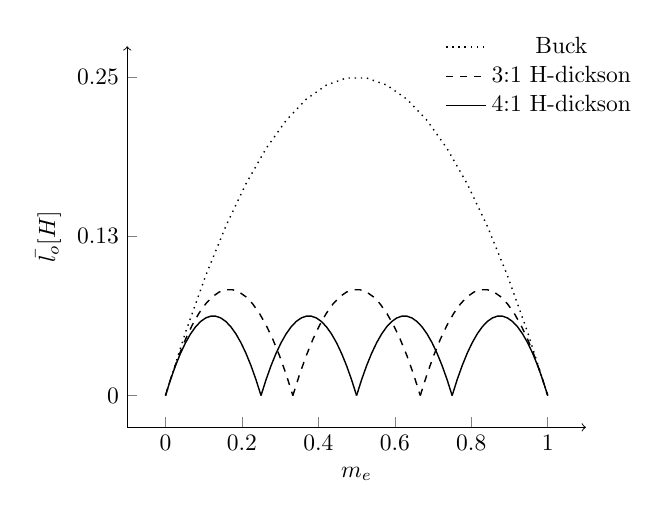
\begin{tikzpicture}[scale=0.85]
    \begin{axis}[
        xlabel near ticks,
        xlabel=$m_e$,
        ylabel={$\bar{l_o}  [ H ]  $} ,
        axis line style={->},
        axis y line*=left,
        axis x line*=bottom,
        ytick = {0,.125,.25},
        %yticklabels={0,$v_{src}\frac{1}{3}$,$v_{src}\frac{2}{3}$,$v_{src}$},
        domain=0:1,
        samples=20,
        %xticklabels={0,$D \cdot T_{sw}$,$T_{sw}$ ,$2 T_{sw}$,$3 T_{sw} $},
        legend style={at={(1.125,1.05)}, anchor= north east,draw=none},
        ]

  \addplot [semithick,dotted] {x*(1-x)};
  \addplot [domain = 0:1/3,  semithick,dashed]   {1/3* (x*3)*(1-(x*3))};
  \addplot [domain = 0:1/4,    semithick]   {1/4* (x*4)*(1-(x*4))};

  \addplot [domain = 1/3:2/3,semithick,dashed] {1/3* (2-x*3)*(1-(2-x*3))};
  \addplot [domain = 2/3:1,  semithick,dashed]   {1/3* (x*3-2)*(1-(x*3-2))};


  \addplot [domain = 1/4:2/4,  semithick]   {1/4* (x*4 - 1)*(1-(x*4 - 1))};
  \addplot [domain = 2/4:3/4,  semithick]   {1/4* (3 - x*4)*(1-(3 - x*4))};
  \addplot [domain = 3/4:4/4,  semithick]   {1/4* (x*4-3)*(1-(x*4-3))};

  \legend {Buck, 3:1 H-dickson,4:1 H-dickson};
\end{axis}
\end{tikzpicture}
\caption{Inductance value for Buck, 3:1 H-Dickson and 4:1 H-Dickson converters as function of the conversion ratio; results are normalized  for $V_{src} = 1V$, $T_{sw}=1s$ and $\Delta i = 1A$.}
\label{fig:inductor_size}
\end{SCfigure}

The reduction in inductance value with respect to the buck converter spans out from $50\%$ conversion ratio to the extremes where the inductance takes the same values for all the converters. The physical size of the inductor is proportional to the peak energy stored in it, and it can be computed from the maximum current through the inductor
\begin{equation}
 E_{l,max}  = \frac{1}{2} i_{max}^2 l_{o}.
\label{eq:eng_L}
\end{equation}
The minimum inductance value occurs when the converter operates in boundary conduction mode (BCM) for converters designed to operate continuous conduction mode (CCM), as is the case of the H-SCC. When a buck or H-SCC converter operates in BCM, the minimum current is equal to zero and the peak current is equal to twice of the output current of the converter. Thus, the maximum inductor current is
\begin{equation}
 i_{max} = \Delta i  = 2 i_{out}
\label{eq:i_max}
\end{equation}
By substituting (\ref{eq:i_max}) and (\ref{eq:buck_l}) into (\ref{eq:eng_L}), the inductor peak energy for a buck can be found
\begin{equation}
E_{l,buck}  =   \frac{ i_{out} v_{src}  D(1-D)}{f_{sw}}.
\label{eq:e_lmax_buck}
\end{equation}
\begin{SCfigure}[][!h]
\centering
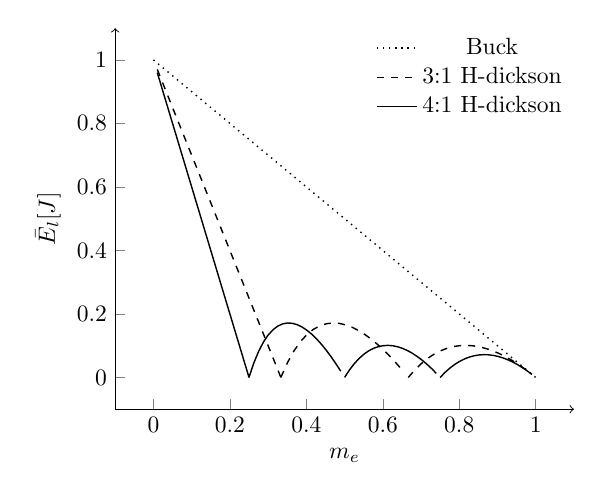
\begin{tikzpicture}[scale=0.85]
    \begin{axis}[
        xlabel near ticks,
        xlabel=$m_e$,
        ylabel={$\bar{E}_{l} [ J ]  $} ,
        axis line style={->},
        axis y line*=left,
        axis x line*=bottom,
        %ytick = {0,.125,.25},
        %yticklabels={0,$v_{src}\frac{1}{3}$,$v_{src}\frac{2}{3}$,$v_{src}$},
        domain=0:1,
        samples=20,
        %xticklabels={0,$D \cdot T_{sw}$,$T_{sw}$ ,$2 T_{sw}$,$3 T_{sw} $},
        legend style={at={(1,1)}, anchor= north east,draw=none},
        ]

  \addplot [semithick,dotted] {(1-x)};
  \addplot [domain = 0.01:1/3, semithick, dashed]   {1/x* 1/3* (x*3)*(1-(x*3))};
  \addplot [domain = 0.01:1/4, semithick]   {1/x* 1/4* (x*4)*(1-(x*4))};

  \addplot [domain = 1/3:2/3-0.01,semithick,dashed] {1/x*1/3* (2-x*3)*(1-(2-x*3))};
  \addplot [domain = 2/3:1-0.01,  semithick,dashed]   {1/x*1/3* (x*3-2)*(1-(x*3-2))};


  \addplot [domain = 1/4:2/4-0.01,  semithick]   {1/x*1/4* (x*4 - 1)*(1-(x*4 - 1))};
  \addplot [domain = 2/4:3/4-0.01,  semithick]   {1/x*1/4* (3 - x*4)*(1-(3 - x*4))};
  \addplot [domain = 3/4:4/4-0.01,  semithick]   {1/x*1/4* (x*4-3)*(1-(x*4-3))};

  \legend {Buck, 3:1 H-dickson,4:1 H-dickson};
\end{axis}
\end{tikzpicture}
\caption{Peak energy storage for Buck, 3:1 H-Dickson, and 4:1 H-Dickson converters as function of the conversion ratio;  results are normalized for $P_{out} = 1W$ and $f_{sw}=1Hz$.}
\label{fig:inductor_energy}
\end{SCfigure}
In a buck converter the source voltage can be written as
\begin{equation}
v_{src}  =  \frac{v_{out}} {D},
\label{eq:vo_buck}
\end{equation}
thus by substituting (\ref{eq:vo_buck}) into (\ref{eq:e_lmax_buck}), the $E_{l,buck}$ yields to
\begin{equation}
E_{l,buck}  =  \frac{v_{vout}}{D} \frac{ i_{out}  D(1-D)}{f_{sw}} = \frac{(1-D)}{f_{sw}} P_{out}.
\label{eq:e_lmax_buck_II}
\end{equation}
By substituting (\ref{eq:i_max}) and (\ref{eq:hscc_l}) into (\ref{eq:eng_L}), the inductor peak energy for a H-SCC using Dickson or Ladder stages can be found
\begin{equation}
E_{l,hscc}  =   \frac{ m_{i} ~ i_{out} ~ v_{src} ~ D(1-D)}{f_{sw}}.
\label{eq:e_lmax_hscc}
\end{equation}
Rearranging~\eqref{eq:eff_m} $v_{src}$ can be written as function of the \emph{effective} conversion ratio, as   
\begin{equation}
v_{src}  =  \frac{v_{out}} {m},
\label{eq:vo_hscc}
\end{equation}
. Thus by substituting (\ref{eq:vo_hscc}) into (\ref{eq:e_lmax_hscc}), the resulting expression of the inductor maximum energy yields to
\begin{equation}
E_{l,hscc}  =  \frac{v_{vout}}{m_e} \frac{ m_i ~i_{out} ~ D(1-D)}{f_{sw}} = \frac{m_i~ D (1-D)}{m_e~ f_{sw}} P_{out}.
\label{eq:e_lmax_hscc_II}
\end{equation}

Figure~\ref{fig:inductor_energy} plots (\ref{eq:e_lmax_buck_II}) and (\ref{eq:e_lmax_hscc_II}), both plots have the same trend of reducing the peak energy as the conversion ratio increases. With regard to the inductance value (see Figure~\ref{fig:inductor_size}), the peak energy stored in the inductor, and hence the volume, are dramatically reduced in case of using a H-SCC topology; as shown in Figure~\ref{fig:inductor_normal}. The plot shows that the reduction in inductance volume ranges from a conversion ratio of $50\%$ to the extremes $0\%$ and $100\%$ symmetrically, being very effective in most of the conversion ratio range of the converter and decreasing at the two extremes. As the intrinsic conversion ratio $m_i$ of the SCC stages decreases, the reduction in inductance increases, and  the effective region spans for a larger range of conversion ratios.
\begin{SCfigure}[][!h]
\centering
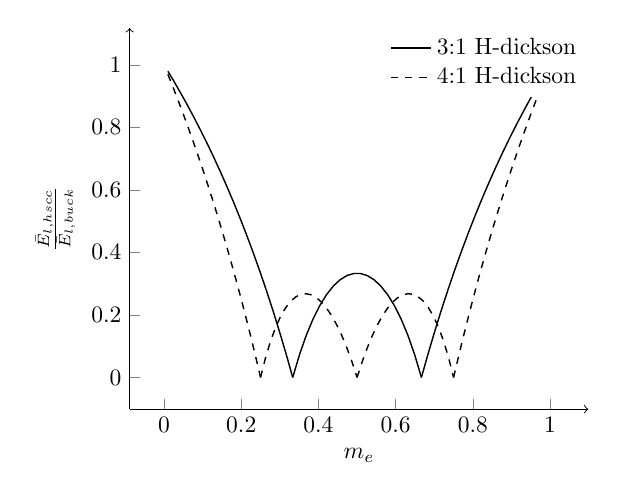
\begin{tikzpicture}[scale=0.85]
    \begin{axis}[
        xlabel near ticks,
        xlabel=$m_e$,
        ylabel={$ \frac{\bar{E}_{l,hscc}}{\bar{E}_{l,buck}}  $} ,
        axis line style={->},
        axis y line*=left,
        axis x line*=bottom,
        %ytick = {0,.125,.25},
        %yticklabels={0,$v_{src}\frac{1}{3}$,$v_{src}\frac{2}{3}$,$v_{src}$},
        domain=0:1,
        samples=20,
        %xticklabels={0,$D \cdot T_{sw}$,$T_{sw}$ ,$2 T_{sw}$,$3 T_{sw} $},
        legend style={at={(1,1)}, anchor= north east,draw=none},
        ]


  \addplot [domain = 0.01:1/3,  semithick]   { (1/x* 1/3* (x*3)*(1-(x*3)))/(1-x) };
  \addplot [domain = 0.01:1/4,    semithick,dashed]   { (1/x* 1/4* (x*4)*(1-(x*4)))/(1-x)};

  \addplot [domain = 1/3:2/3,semithick] { (1/x*1/3* (2-x*3)*(1-(2-x*3)))/(1-x)};
  \addplot [domain = 2/3:1,  semithick]   { (1/x*1/3* (x*3-2)*(1-(x*3-2)))/(1-x)};


  \addplot [domain = 1/4:2/4,  semithick,dashed]   { (1/x*1/4* (x*4 - 1)*(1-(x*4 - 1)))/(1-x)};
  \addplot [domain = 2/4:3/4,  semithick,dashed]   { (1/x*1/4* (3 - x*4)*(1-(3 - x*4)))/(1-x)};
  \addplot [domain = 3/4:4/4,  semithick,dashed]   { (1/x*1/4* (x*4-3)*(1-(x*4-3)))/(1-x)};

  \legend {3:1 H-dickson,4:1 H-dickson};
\end{axis}
\end{tikzpicture}
\caption{Peak energy storage normalized with respect to a buck converter for a 3:1 H-Dickson and a 4:1 H-Dickson converters as function of the conversion ratio.}
\label{fig:inductor_normal}
\end{SCfigure}

\subsection{Power Switches}
The large number of switches used in a H-SCC has different advantages with regards to miniaturization of the converter. In fact, in a H-SCC the voltage stress applied to the different switches is a fraction of the input voltage, in contrast to the buck converter where each of the switches have to block the full input voltage. Therefore SCCs can be implemented with switches rated at lower voltages than the input voltage. Table ~\ref{tab:3:1 H-Dick_V_stress} shows the blocking voltages of the switches of the 3:1 H-Dickson of Figure~\ref{fig:3_1_hscc}. Reducing the voltage stress at the switches the following advantages:
\begin{itemize}
  \item Low voltage devices take less silicon area in the standard integration processes.
  \item Switching performance of these devices is better since they are smaller in area, and with less parasitic capacitances, as a consequence, they can switch faster.
  \item Switching losses of the converter are reduced since they have a quadratic relationship with the blocking voltages of the switches ($v_{ds}$).
\end{itemize}
From the three above-mentioned advantages, the two first facts are mainly technology-related hence their benefits are not trivial to be quantified. In contrast, the last fact can be assumed to be technology-independent and easily quantified. By assuming that drain-source capacitance $c_{ds}$ is a constant among different devices and technologies, the switching losses can be computed and compared with respect to the buck. 
\begin{table}[h]
\centering
\caption{Stress voltages at the switches of the 3:1 H-Dickson of Figure~\ref{fig:3_1_hscc}.}
\label{tab:3:1 H-Dick_V_stress}
\renewcommand{\arraystretch}{1.5}% Wider
\begin{tabular}{r  c}
 Switch & $v_{ds}$  \\
 \midrule
 $s_1,s_3 \cdots s_7$ & $\frac{1}{3} v_{src}$ \\
 $s_2$ & $\frac{2 }{3} v_{src}$
\end{tabular}
\end{table}
Switching losses are given by~\cite{2001Erickson}
\begin{equation}
P_{sw} = \frac{1}{2} f_{sw} \cdot c_{ds} \cdot v_{ds}^2.
\label{eq:p_sw_dev}
\end{equation}
In a buck converter of Figure~\ref{fig:ind_ckt_l} the blocking voltage of the switches is $v_{src}$, thus using~\eqref{eq:p_sw_dev} the switching losses result in
\begin{equation}
P_{sw,buck} =   f_{sw} \cdot c_{ds} \cdot v_{src}^2.
\label{eq:p_sw_buck}
\end{equation}
The blocking voltages of the 3:1 H-Dickson are in table~\ref{tab:3:1 H-Dick_V_stress}, thus applying~\eqref{eq:p_sw_dev}) the switching losses in this case results in
\begin{equation}
P_{sw,hscc} =  \frac{6}{2}  f_{sw} \cdot c_{ds} \left( \frac{1}{3} v_{src} \right)^2 + \frac{1}{2}  f_{sw} \cdot c_{ds} \left( \frac{2}{3} v_{src} \right)^2 ,
\label{eq:p_sw_hscc}
\end{equation}
rearranging~\eqref{eq:p_sw_hscc},  yields to
\begin{equation}
P_{sw,hscc} =  \frac{5}{9}  f_{sw} \cdot c_{ds} \cdot v_{src}^2.
\label{eq:p_sw_hscc_sol}
\end{equation}
Dividing (\ref{eq:p_sw_buck}) and (\ref{eq:p_sw_hscc_sol}) yields ratio between the two converters
\begin{equation}
\frac{P_{sw,hscc}}{P_{sw,buck}} =  \frac{5}{9},
\label{eq:p_sw_rel}
\end{equation}
thus achieving a reduction of almost one half with respect to the buck converter, even when the H-SCC converter is using five more switches than the buck converter. Applying~\eqref{eq:p_sw_dev} with the blocking voltages defined for the N:1 Dickson and Ladder converters in Table~\ref{tab:Dick_Ladder_v_blk}, the formulation of the switching losses can be generalized, resulting in
\begin{align}
P_{sw,dickson} & =  \frac{4+N}{8 \cdot N^2} \cdot v_{vin}^2 \cdot f_{sw}  \cdot {c_{ds}} , \\
P_{sw,ladder}  & =  \frac{1}{ N} \cdot v_{src}^2 \cdot f_{sw} \cdot {c_{ds}}    .
\label{eq:p_sw_gen}
\end{align}
Normalizing them with respect to the power losses of the buck converter~\eqref{eq:p_sw_buck}, yields
\begin{align}
\bar{P}_{sw,dickson} & = \frac{4+N}{8 \cdot N^2} ,\label{eq:n_sw_dick}\\
\bar{P}_{sw,ladder} & = \frac{1}{ N}. \label{eq:n_sw_lddr}
\end{align}
\begin{table}[h]
\centering
\caption{Switch blocking voltage of Dickson and Ladder converters.}
\label{tab:Dick_Ladder_v_blk}
\renewcommand{\arraystretch}{1.5}% Wider
\begin{tabular}{r | c  c   }
 Converter &  N:1 Dickson  $ N \geq$ 3  &  N:1 Ladder $ N \geq 2$  \\
 \midrule
\# Switches & $ 4 + N $  & $2 \cdot N$ \\
 $v_{ds}$ &     $\begin{array} {rcl} 6   & \to &  \frac{v_{src}}{N} \\
                                     (N - 2) & \to & \frac{2 v_{src}}{N}   
                 \end{array}$
          &  $\frac{v_{src}}{N} $ \\
\end{tabular}
\end{table}

Figure~\ref{fig:psw_ratio} plots~\eqref{eq:n_sw_dick} and~\eqref{eq:n_sw_lddr }, showing the switching loss ratio with respect to the buck converter. It can be seen that both converters reduce the switching losses with respect to the buck converter. In fact, as $N$ increases to losses decrease, although the number of switches increase as well. Reducing the switching loss will enable to operate the converter at higher frequencies, thus with a smaller switching period $T_{sw}$, which is also effective in the reduction of the power inductor. 

\begin{SCfigure}
\centering
\begin{tikzpicture}[scale=0.7]
    \begin{axis}[
        xlabel near ticks,
        xlabel=$N$,
        ylabel=$P_{sw}/P_{sw,buck}$,
        axis line style={->},
        axis y line*=left,
        axis x line*=bottom,
        domain=3:10,
        samples=7,
        legend style={
                draw=none,}
        ]
  %\addplot [semithick] {x*0+1};
  \addplot [semithick,smooth,mark=o,mark size=2,scale plot marks=false] {(4+x)/(8*x^2)};
  \addplot [semithick,smooth,mark=square, mark size=2 ,scale plot marks=false]{1/x};
  \legend {Dickson,Ladder};
\end{axis}
\end{tikzpicture}
\caption{Switching loss ratio for Dickson and Ladder converters with respect to the buck converter.}
\label{fig:psw_ratio}
\end{SCfigure}

The lecture of the results is given from a qualitative perspective, consequently a couple of considerations are given regarding a practical implementation of a H-SCC. First, they are obtained assuming that $c_{ds}$ is the same for all the switches in both converters. In a practical converter each device has a different $c_{ds}$ value defined by two of the device parameters; $c_{ds}$ is directly proportional to the rated $v_{ds}$  voltage and inversely proportional to the channel resistance $r_{on}$. Theoretically, lower voltage switches have smaller $c_{ds}$, but the final value will also depend on its $r_{on}$. Second, H-SCC has a larger number of devices in series in the current path compared to a buck, that only has only one switch in the current path in both phases. A proper H-SCC design reduces the number of switches in the high current path, helping to keep the conduction loss low.

\subsection{Multiple Outputs}
The use of the internal nodes of the SCC allows to provide multiple outputs with a single power train. In this case the converter could be simultaneously loaded at the \emph{pwm}-nodes and at the \emph{dc}-node, providing different conversion ratios for each output. The conversion ratio at the \emph{dc}-node (or nodes)  is given by the intrinsic conversion ratio of the converter $m_i$, independent of the variations in the duty cycle of the driving signal, yet this fixed output can be linearly regulated to adjust the output voltage.  The conversion ratio for the other \emph{pwm}-nodes is a function of $D$ and determined for each node by the node conversion ration $m_n$. In the case of using multiple \emph{pmw}-nodes, all the outputs will depend on $D$, hence it will not be possible to have independent regulation for each of the outputs. This happens because in order to guarantee the proper operation of a SCC, all switches are associated to a phase, hence they can not be independently controlled.
\begin{figure}[!h]
\centering
\ctikzset { bipoles/length=1cm}
\begin{circuitikz}[american voltages,scale=0.65]
\draw
        %Draw Switches

        (0,0) node[sground]{} to[V=$v_{src}$]
        (0,8)  --
        (5,8)   to[switch,l_=$s_1$,]
        (5,6)   to[switch,l_=$s_2$]
        (5,4)   to[switch,l_=$s_3$]
        (5,2)   to[switch,l_=$s_4$]
        (5,0)  --
        (0,0)

        (5,6) to[short] (8,6) to[L,l=$l_o$] (12,6) to[C,l_=$c_o$] (12,3) node[sground]{}
        (11,6) -- (14,6) to[R,l_=$r_2$,v^=$v_{o2}$] (14,3) node[sground]{}

        (5,4) to[short]
        (9,4) to[R,l_=$r_1$,v^=$v_{o1}$] (9,0) -- (5,0)

%Draw Capacitors
        (5,2) --
        (3,2) to[C=$c_{fly}$]
        (3,6)--
        (5,6)

        (5,0) --
        (7,0) to[C,l=$c_{dc}$]
        (7,4)--
        (5,4);

\end{circuitikz}
\caption[Two output H-SCC]{2:1 H-SCC with two outputs; $r_1$ is supplied by the \emph{dc}-node and $r_2$ is supplied by the first \emph{pwm}-node.}
\label{fig:2:1hscc_dual_output}
\end{figure}

Figure~\ref{fig:2:1hscc_dual_output} shows a converter with two output voltages. One load $r_1$ is connected to the \emph{dc}-node with an output voltage approximated by
\begin{equation}
v_{o1} = \frac{1}{2} v_{src}.
\end{equation}
the other load $r_2$ is connected to the first \emph{pwm}-node with an output voltage function of $D$ as
\begin{equation}
v_{o2} = \frac{1+D}{2} v_{src}.
\end{equation}
The voltage $v_{o2}$ can be regulated by means of $D$.

\section{DC-DC LED Drivers}
The buck converter is one of the most used topologies for LED drivers in \emph{dc-dc} applications. It has an excellent current regulation and a continuous output current thanks to the inductor connected in series with the output, as shown in Figure~\ref{fig:ind_ckt_led_drv}.

\begin{figure}[!h]
\centering
\ctikzset { bipoles/length=1cm}
\begin{subfigure}[t]{.45\textwidth}
    %\centering
    \raggedright
    \begin{circuitikz} [american voltages,scale=0.65]
    \draw
        (-1,0) to[V = $v_{src}$]
        (-1,4) -- (1,4) to[switch,l_=$s_1$]
        (1,2) -- (1.5,2) to[inductor=${l_o}$,i=$i_o$]
        (3.5,2) -- (4,2) to[C,l_=$c_o$] (4,0) -- (-1,0);

    \draw (4,2) to[short] (5.5,2) to[leD*,v_=$v_o$] (5.5,0) -- (4,0);

    \draw (1,2) to[switch,l_=$s_2$] (1,0);

    \draw (1,2) node[anchor=east] {$v_x$};

    \draw (0,-1) node[anchor=south] {};

    \end{circuitikz}
    \caption{}
    \label{fig:ind_ckt_led_drv}
\end{subfigure}
\hfill
\begin{subfigure}[t]{.45\textwidth}
    %\centering
    \raggedleft
    \begin{circuitikz} [scale=0.65]
    \begin{scope}%[xshift = 8cm, yshift=0cm]
        \draw[->] (0,0) -- (6.25,0) node[anchor=north] {$  t $};
        \draw[->] (0,0) -- (0,3.2) node[anchor= east] {$v_x $};

        %Ticks X
        \draw (2.75,2pt) -- (2.75,-5pt) node[anchor=north] {$T$};
        \draw (5.5,2pt) -- (5.5,-5pt) node[anchor=north] {$2T$};

        %Ticks Y
        \draw (2pt,2.5) -- (-5pt,2.5) node[anchor=east] {$v_{src}$};
        \draw (0,0) node[anchor=north east] {$0$};


        \draw[thick] (0,2.5) -- (1.25,2.5) -- (1.25,0) -- (2.75,0) -- (2.75,2.5) -- (4,2.5) -- (4,0) -- (5.5,0);
        \draw (0,-1) node[anchor=south] {};

        \draw[pil,>-<] (4.78,1.65) -- (4.78,0.6);
        \draw (4.78,0.55) -- (4.78,1.85)node[anchor=west] {$\Delta v_f$};



        \draw[thick,dotted] (0,1.36) -- (6,1.36) ;
        \draw[thick,dotted] (0,0.9) -- (6,0.9) ;
        \draw[thick,dashed] (0,1.137) -- (6,1.137) node[anchor=west] {$\bar{v_o}$};

    \end{scope}
    \end{circuitikz}
    \caption{}
\label{fig:induc_vx_led_drv}
\end{subfigure}
\caption[Switching node in the buck]{\emph{Left} - buck based LED driver schematic; \emph{right} - transient voltage at the switching node(thick line), average output voltage (dashed line), and forward voltage limits (dotted lines). }
\label{fig:inductive_led_drv}
\end{figure}

It can be seen in Figure~\ref{fig:induc_vx_led_drv} that the voltage swing at the switching node ($v_x$) of a buck converter goes from ground to $v_{src}$ providing the full conversion ratio range, between 0 and 1. Actually, this regulation range is often much wider than the margins of variation in the LED's forward voltage, as shown in Figure~\ref{fig:induc_vx_led_drv}. The \emph{dashed} line represents the average output voltage $\bar{v_o}$, thus the LED's forward voltage $v_f$, and the dotted lines represent the forward voltage variation boundaries $\Delta v_f$, being them around $\pm10\%$. Previously, in Chapter~\ref{sc:LED_load} was given a detailed discussion about the characteristics of the LED as a load.

\begin{figure}[!h]
\centering
\ctikzset { bipoles/length=1cm}
\begin{subfigure}[t]{.45\textwidth}
    %\centering
    \raggedright
    \begin{circuitikz} [american voltages,scale=0.65]
    \draw[dotted] (1,4) -- (1,3.5);

    \draw (1,3.35) -- (0.5,3.35);
    \draw[dotted] (0.5,3.35) --  (-.25,3.35) -- (-.25,3);

    \draw
        (1,3.5) to[switch,l_=$s_2$]
        (1,2) -- (2,2) to[inductor=${l_o}$,i=$i_o$]
        (4,2) -- (4,2) to[C,l_=$c_o$] (4,0.5) node[sground]{};

    \draw (4,2) to[short] (5.5,2) to[leD*,v_=$v_o$] (5.5,0.5) node[sground]{};

    \draw (1,2) to[switch,l_=$s_3$] (1,0.5);
    \draw[dotted] (1,0.5) --  (1,0) ;

    \draw (1.75,2) -- (1.75,1.5);
    \draw[dotted] (1.75,1.5) -- (1.75,1);

    \draw (1,2) node[anchor=east] {$v_x$};

    \draw (0,-1) node[anchor=south] {};

    \end{circuitikz}
    \caption{}
    \label{fig:hscc_ckt_led_drv}
\end{subfigure}
\hfill
\begin{subfigure}[t]{.45\textwidth}
    %\centering
    \raggedleft
    \begin{circuitikz} [scale=0.65]
    \begin{scope}%[xshift = 8cm, yshift=0cm]
        \draw[->] (0,0) -- (6.25,0) node[anchor=north] {$  t $};
        \draw[->] (0,0) -- (0,3.2) node[anchor= east] {$v_x $};

        %Ticks X
        \draw (2.75,2pt) -- (2.75,-5pt) node[anchor=north] {$T$};
        \draw (5.5,2pt) -- (5.5,-5pt) node[anchor=north] {$2T$};

        %Ticks Y
        \draw (2pt,2.5) -- (-5pt,2.5) node[anchor=east] {$v_{src}$};
        \draw (2pt,1.67) -- (-5pt,1.67) node[anchor=east] {$v_{src} \frac{2}{3}$};
        \draw (2pt,0.83) -- (-5pt,0.83) node[anchor=east] {$v_{src} \frac{1}{3}$};
        \draw (0,0) node[anchor=north east] {$0$};


        \draw[thick] (0,1.67) -- (1.25,1.67) -- (1.25,0.83) -- (2.75,0.83) -- (2.75,1.67) -- (4,1.67) -- (4,0.83) -- (5.5,0.83);
        \draw (0,-1) node[anchor=south] {};

        \draw[pil,>-<] (4.78,1.65) -- (4.78,0.6);
        \draw (4.78,0.55) -- (4.78,1.85)node[anchor=west] {$\Delta v_f$};



        \draw[thick,dotted] (0,1.36) -- (6,1.36) ;
        \draw[thick,dotted] (0,0.9) -- (6,0.9) ;
        \draw[thick,dashed] (0,1.137) -- (6,1.137) node[anchor=west] {$\bar{v_o}$};

    \end{scope}
    \end{circuitikz}
    \caption{}
\label{fig:hscc_vx_led_drv}
\end{subfigure}
\caption[Switching node in the H-SCC]{\emph{Left} - switching node detail of a 3:1 H-Dickson based LED driver; \emph{right} - transient voltage at the switching node(thick line), average output voltage (dashed line), and forward voltage limits (dotted lines).  }
\label{fig:hscc_led_drv}
\end{figure}

The abrupt $v-i$ characteristics of the LEDs is an advantage for the reduced conversion range of the H-SCC. Contrary to the buck converter, the H-SCC has a smaller voltage swing in the switching node. Figure~\ref{fig:hscc_led_drv} shows that the voltage limits of the switching node in a H-SCC can accommodate $\Delta v_f$ variations of the LED load.  As previously described in Section~\ref{sec:out_reg}, the dynamic conversion range at the outputs depend on the intrinsic conversion ratio $m_i$ of the SCC stage, therefore it can be adjusted for the requirements of the load.

%The following subsections present different LED drivers based on H-SCCs for \emph{dc-dc} and \emph{ac-dc}. The presented topologies are also suitable to supply other load types, specially when these require a reduced conversion margin.

\subsection{Single-stage \emph{dc-dc} with auxiliary output voltage}
\begin{figure}[!h]
\ctikzset { bipoles/length=1cm}
\centering
    \begin{circuitikz}[american voltages,scale=0.6]

    \draw
            %Input Supply
            (0,0)  to[V=$v_{src}$]
            %Draw Switches
            (0,10.5)  --
            (5,10.5)  to[switch=$s_1$] %node[anchor=west] {$n_1$}%S1
            (5,9)  to[switch=$s_2$] %node[anchor=east] {$n_2$}%S1
            (5,7.5)  to[switch=$s_3$] %node[anchor=east] {$n_3$}%S1
            (5,6)   to[switch=$s_4$] %node[anchor=west] {$n_4$}%S2
            (5,4.5)   to[switch=$s_5$] %node[anchor=west] {$n_5$}%S3
            (5,3) --
            %left branch
            (3,3)   to[switch=$s_9$]
            (3,1.5)   to[switch=$s_8$]
            (3,0);

    \draw   %right branch
            (5,3) --
            (7,3)   to[switch,l_=$s_6$]
            (7,1.5)   to[switch,l_=$s_7$]
            (7,0) -- (0,0);



    \draw %Capacitor C1
           (2,6)
            to[pC,l_=$c_1$] (2,9) --
           (5,9);

    \draw %Capacitor C2
           (8.25,4.5)  to[pC,l_=$c_2$](8.25,7.5) --
           (5,7.5);

    \draw %Capacitor C3
           (3,1.5) -- (2,1.5)
            to[pC,l_=$c_3$] (2,6) --
           (5,6);

    \draw %Capacitor C4
           (7,1.5) --
           (8.25,1.5) -- (8.25,3) to[pC,l_=$c_4$](8.25,4.5) --
           (5,4.5);


    \draw  %LC output filter &  Output LED string
            (8.25,7.5)node[anchor=south] {$v_x$} to[L=$l_o$] (14,7.5)
            (13.5,0) to[pC,l=$c_{o}$] (13.5,7.5) -|
            (16,7.5) -- (16,7)  to[leD*] (16,5) to[leD*] (16,3) to[leD*] (16,1)   |- (7,0) ;

    %Vout label
    \draw (16.25,8.5) to[open,v^=$v_{out}$] (16.25,-1);

    \draw %Capacitor C3
           (5,0) to[pC,l_=$c_5$] (5,3) ;% node[anchor=south east] {$n_{dc}$};

     %\draw (7,4) to[short,-o] (10,4) node[anchor=west] {};
     %\draw (7,0) to[short,-o] (12,0) node[anchor=west] {};


     \draw (7,3) --([hs]8.25,4 |- 7,3) arc(180:0:\radius) to[short,-o] (10,3) to[open,v^=$v_{aux}$] (10,0) ;


     \end{circuitikz}
 \caption[5:1 H$^2$-Dickosn 12W LED driver]{ 5:1 H$^2$-Dickson LED driver for 24V e-merge track lighting application. The driver has two outputs: A $12V$, $12W$  LED string, and $4V$, $200mW$  to supply low power auxiliary loads. }
 \label{fig:5_1_hscc_emerge}
\end{figure}
Figure~\ref{fig:5_1_hscc_emerge} shows the \emph{dc-dc} LED driver with an auxiliary output voltage~\cite{WO2015/040564}.
In fact, this architecture has been used in an experimental set-up for this dissertation presented in the last chapter. The converter features two outputs: The main output $v_{out}$ supplies the LED load and normally delivers the largest amount of power. The output voltage can be controlled using the duty cycle $D$, thus its value is given by
\begin{equation}
v_{out} =  v_{src}  \frac{4 - D }{5}.
\label{eq:dc_dc_vout}
\end{equation}
The secondary output $v_{aux}$ supplies the low voltage electronics dedicated to the control of the driver, providing functionalities such as connectivity, light control and stand-by operation. The secondary output has no direct means of regulation and provides a fix conversion ratio equal to
\begin{equation}
v_{aux} =  v_{src} \frac{1 }{5}.
\label{eq:dc_dc_vaux}
\end{equation}
Nevertheless, the voltage at this output can still be controlled by means of a linear regulator.
\begin{figure}[!h]
\ctikzset { bipoles/length=1cm}
\centering
    \begin{circuitikz}[american voltages,scale=0.6]

    \draw
            %Input Supply
            (0,0)  to[V=$v_{src}$]
            %Draw Switches
            (0,10.5)  --
            (5,10.5)  to[switch=$s_1$] %node[anchor=west] {$n_1$}%S1
            (5,9)  to[switch=$s_2$] %node[anchor=east] {$n_2$}%S1
            (5,7.5)  to[switch=$s_3$] %node[anchor=east] {$n_3$}%S1
            (5,6)   to[switch=$s_4$] %node[anchor=west] {$n_4$}%S2
            (5,4.5)   to[switch=$s_5$] %node[anchor=west] {$n_5$}%S3
            (5,3) --
            %left branch
            (3,3)   to[switch=$s_9$]
            (3,1.5)   to[switch=$s_8$]
            (3,0);

    \draw   %right branch
            (5,3) --
            (7,3)   to[switch,l_=$s_6$]
            (7,1.5)   to[switch,l_=$s_7$]
            (7,0) -- (0,0);



    \draw %Capacitor C1
           (2,6)
            to[pC,l_=$c_1$] (2,9) --
           (5,9);

    \draw %Capacitor C2
           (8.25,4.5)  to[pC,l=$c_2$](8.25,7.5) --
           (5,7.5);

    \draw %Capacitor C3
           (3,1.5) -- (2,1.5)
            to[pC,l_=$c_3$] (2,6) --
           (5,6);

    \draw %Capacitor C4
           (7,1.5) --
           (8.25,1.5) -- (8.25,3) to[pC,l=$c_4$](8.25,4.5) --
           (5,4.5);


    \draw  %LC output filter &  Output LED string
            (12,7.5)node[anchor=south west] {$v_x$} to[L=$l_o$] (15.5,7.5)
            (15,0) to[pC,l=$c_{o}$] (15,7.5) -|
            (16.5,7.5) -- (16.5,7)  to[leD*] (16.5,5) to[leD*] (16.5,3) to[leD*] (16.5,1)   |- (7,0) ;

            %Mux
    \draw   (12,7.5) -- (12,8.5) -- (11,9) -- (11,6) -- (12,6.5) -- (12,7.5)
            (11.5,7.5) node[rotate=90] {$mux$}
            (11.5,8.75) -- (11.5,9.5) node[anchor=west, rotate=90] {$sel$};

    \draw    %Mux connections
            (5,9)  --  (10,9) |- (11,8.5)
            (8.25,7.5)  --  (11,7.5)
            (5,6) --  (6.5,6) -- ([vs_d]5,7.5 -| 6.5,8 ) arc(270:90:\radius) --  (6.5,8) -- (11,8)
            (8.25,4.5) -| (9.5,7) -- (11,7)
            (8.25,1.5) -| (10,6.5) -- (11,6.5);

    %Vout label
    \draw (17,9) to[open,v^=$v_{out}$] (17,-1);

    \draw %Capacitor C3
           (5,0) to[pC,l_=$c_5$] (5,3) ;% node[anchor=south east] {$n_{dc}$};

     \end{circuitikz}
 \caption[5:1 H-Dickson LED driver 24V-12V-4V 12W LED driver]{ 5:1 H-Dickson LED driver with a multiplexer that enables to connect the different switching nodes with the power inductor.  }
 \label{fig:5_1_hscc_mux}
\end{figure}

\subsection{Single-stage \emph{dc-dc} with extended conversion range }

The reduced voltage swing at $v_x$, on the one hand favors in the reduction of output inductor, but on the other hand shrinks the conversion to a narrow range between $3/5$ and $4/5$. Using the same topology, the conversion ratio of the converter can be extended to the full range between 0 and 1, like in a buck converter, introducing a multiplexer~\cite{WO2015/040517} between the different floating \emph{pwm}-nodes and the power inductor as shown in Figure~\ref{fig:5_1_hscc_mux}. With this enhancement the power inductor can now be connecter to any of the available \emph{pwm}-nodes of the SCC stage.
%A detailed description of this architecture can be found in the annex X section Y.


\section{Summary}

In this chapter the hybrid switched capacitor converter (H-SCC) was introduced. First, the main operation and performance characteristics of the SCC were presented, with special emphasis on the limitations that these converters have with respect to load  regulation.

Subsequently, the H-SCC was described as a combination of SCC with an inductor. Such a \emph{hybrid} combination makes it possible to achieve a much better regulation than possible with the pure SCCs. In fact, the regulation enhancements in the H-SCC make the converter comparable to an inductive converters, especially to the buck. For that reason, two metrics were presented in order to qualitatively evaluate the benefits of these converters with respect to integration. These metrics shown that when using a H-SCC the inductor size and switching losses can be reduced compared to a buck converter.

Finally, the last section was dedicated to exploring the possibilities of the H-SCCs for LED driving. Different driver architectures for \emph{dc-dc} applications were presented, introducing the architecture that was used in the final demonstrator if this disoperation. 

In conclusion, the H-SCC is a new power converter topology composed of a SCC and an inductor. The SCC implements the power train structure, where the SCC's conversion ratio adds a new variable to the design of the converter. Modifying this variable allows to adjust the voltages stress if the switches, capacitors, and inductors, and favors the integrability of the converter. At the same time, the extra inductor extends the regulation margins because it allows to control the output voltage with the duty cycle of the SCC stage.


\clearpage
\bibliographystyle{plainnat}
\bibliography{references} 